\documentclass{tudscrartcl}

%encoding and language
\usepackage[utf8]{inputenc}
\usepackage[T1]{fontenc}
\usepackage[english]{babel}

%Mathesymbole
\usepackage{amssymb}
\usepackage{amsthm}
\usepackage{amsmath}
\usepackage{mathtools}

%Form
\usepackage{enumerate}
\usepackage{subfig}

%Algorithmus
\usepackage{algorithm}
\usepackage{algorithmicx}
\usepackage{algpseudocode}

%Literatur
\usepackage[backend=biber, style=alphabetic]{biblatex}
\usepackage{csquotes}
\bibliography{../bib/literatur}

%Theorem
\theoremstyle{definition}
\newtheorem{definition}{Definition}[section]
\newtheorem{example}{Example}[section]
\newtheorem{notation}{Notation}[section]
\newtheorem{lemma}{Lemma}[section]
\newtheorem{theorem}{Theorem}[section]
\newtheorem{construction}{Construction}[section]

%Operatoren
\DeclareMathOperator*{\argmax}{argmax}
\DeclareMathOperator*{\argmin}{argmin}

%derivation relation
\newcommand{\rpath}[2]{\xRightarrow{\text{#1}}_{#2}}

%title page
\title{Learning Pruning Policies for Linear Context-free Rewriting Systems}
\subtitle{INF-PM-FPG}
\author{Andy Püschel}
\date{\today}
\faculty{Faculty of Computer Science}
\institute{Theoretical Computer Science}
\chair{Chair of Foundations of Programming}

\begin{document}

\maketitle


\section{Introduction}

Syntactiv parsing is the problem of determining the syntactic structure of a given sentence.
If a sentence can be parsed, the algorithm returns the syntactic structure of the given sentence e.g. in form of derivation trees or even more information about the whole parsing process e.g. in form of parse charts.
One of the parsing algorithms is the weighted deductive parsing algorithm, introduced by \cite{nederhof03}, which takes as input a word and a grammar. 
The weighted deductive parsing algorithm uses different deduction rules to create constituents from single words in the sentence firstly, and secondly from already created constituents. 
Since the runtime varies in the size of the grammar (size of the set of rules), particular grammar constants and the sentence length, pruning policies will be a not indispensable feat. 
A pruning policy decides whether a certain constituent for a part of the sentence is likely to be a good constituent or not.
The application of a given pruning policy can reduce the runtime of a parser drastically.
Nevertheless, a given pruning policy is not always optimal for different sentences generated by the same grammar.

In this paper, we will introduce an approach to train such a pruning policy for PLCFRS.
The main objective of this paper will be to introduce a method similar to \cite{vieira17} but for PLCFRS instead of PCFG.

After considering the prelimniaries in Section 2, we extend the weighted deductive parsing algorithm for PLCFRS by a pruning policy Section 3. In Section 4, the Locally Optimal Learning to Search training algorithm (\textproc{Lols}), introduced by \cite{chang15}, is presented for pruning policies. Furthermore a metric will be provided which asks, how to evaluate (how to reward) a pruning policy. To improve the runtime of the training algorithm, we present the change propagation algorithm, introduced by \cite{vieira17}.
In Section 5, a description for our experimental setup in detail will be given and the results will be presented in Section 6.
At last, we conclude our work in Section 7.


\section{Preliminaries}

To ensure a common understanding of terms, some fundamental definitions and notations will be introduced in this section.
For the formal language theory we use the definitions by \cite{chomsky56} and \cite{lari90}. Firstly, we denote by $\mathbb{N}$ the set of natural numbers.
Now, for each $k \in \mathbb{N}$, we define $[k] = \{1, \ldots, k\}$.

\begin{definition}[Relation Product]
	Let $A, B, C$ be sets
	and $R \subseteq A \times B$, $S \subseteq B \times C$ be relations.
	We define the \emph{relation product} as
	\begin{align*}
		R;S = \{(a,c) \in A \times C \mid
			\exists b \in B: (a,b) \in R \text{ and } (b,c) \in S\}.
	\end{align*}
\end{definition}

\begin{definition}[Alphabet]
	An \emph{alphabet} is a finite nonempty set.
\end{definition}

\begin{definition}[Sentence Length]
	Let $\Sigma$ be an alphabet and $w = w_1 \ldots w_n \in \Sigma^*$.
	The \emph{length of $w$} is defined as $|w| = n$.
\end{definition}

\begin{definition}
	Let $l \in \mathbb{N}$, $X_1, \ldots, X_l$ be nonempty sets,
	$x = (x_1, \ldots, x_l) \in X_1 \times \ldots \times X_l$ be a tuple
	and $i \in [l]$.
	The \emph{$i$-th element of $x$} is denoted by $x|_i = x_i$.
\end{definition}

\begin{definition}[Set of Trees]
	Let $\Sigma$ be an alphabet and $H$ be a set disjoint from $\Sigma$.
	The \emph{set of unranked trees over $\Sigma$ indexed by $H$},
	denoted by $T_{\Sigma}(H)$, is the smallest set $U$ such that:
	\begin{enumerate}[(i)]
		\item $H \subseteq U$
		\item $\forall k \in \mathbb{N}, \sigma \in \Sigma,
			\xi_1, \ldots, \xi_k \in U:
			\sigma(\xi_1, \ldots, \xi_k) \in U$
	\end{enumerate}
	We denote $T_{\Sigma}(\emptyset)$ as $T_{\Sigma}$.
\end{definition}

\begin{definition}[Sorted Set]
	Let $S$ be a countable set (called sorts).
	An \emph{$S$-sorted set} is a tuple $(A, sort)$ where
	\begin{itemize}
		\item $A$ is a set and
		\item $sort: A \to S$.
	\end{itemize}
	$(A, sort)$ is called \emph{finite} if for each $s \in S: A_s$ is finite,
	it is called \emph{nonempty} if $\bigcup_{s \in S}A_s$ is nonempty
	and we write $a \in (A, sort)$ if $a \in A$.
	We denote $(A, sort)$ as $A$.
\end{definition}

\begin{definition}[LCFRS \cite{vshanker87}, \cite{kallmeyer12}]
	A \emph{linear context-free rewriting system} is a tuple
	$G =(N, \Sigma, \Xi, P, S)$ where
	\begin{itemize}
		\item $N$ is a finite nonempty $\mathbb{N}$-sorted set (nonterminal symbols),
		\item $\Sigma$ is a finite set (terminal symbols)
			(with $\forall l \in \mathbb{N}: \Sigma \cap N_l = \emptyset$),
		\item $\Xi$ is a finite nontempty set (variable symbols)
			(with $\Xi \cap \Sigma = \emptyset$ and
			$\forall l \in \mathbb{N}: \Xi \cap N_l = \emptyset$),
		\item $P$ is a \emph{set of production rules}
			of the form $\rho = \phi \to \psi$ where
			\begin{itemize}
				\item $\phi = A(\alpha_1, \ldots, \alpha_l)$
					(called left-hand side of $\rho$)\\
					where $l \in \mathbb{N}$, $A \in N_l$,
					$\alpha_1, \ldots, \alpha_l \in (\Sigma \cup \Xi)^*$ and
				\item $\psi = B_1(X^{(1)}_1, \ldots, X^{(1)}_{l_1})
					\ldots B_m(X^{(m)}_1, \ldots, X^{(m)}_{l_m})$
					(called right-hand side of $\rho$)\\
					where $m \in \mathbb{N}$, $B_1 \in N_{l_1}, \ldots, B_m \in N_{l_m}$,
					$X^{(i)}_{j} \in \Xi$ for $1 \leq i \leq m, 1 \leq j \leq l_i$
			\end{itemize}
			and for every $X \in \Xi$ occurring in $\rho$ we require that $X$ occurs
			exactly once in the left-hand side of $\rho$ and
			exactly once in the right-hand side of $\rho$, and
		\item $S \in N_1$ (initial nonterminal symbol).
	\end{itemize}
	A nonterminal symbol $A \in N$ has \emph{fanout} $l$, denoted by $fanout(A)$, if
	$A \in N_l$. The fanout of a LCFRS $G$ is defined as
	$fanout(G) = \max \bigcup_{A \in N}fanout(A)$.\\
	A LCFRS is called \emph{ordered} if for every
	$\rho = \phi \to \psi \in P$ and for each
	$X_1, X_2 \in V$ occurring in $\phi$ and $\psi:$
	$X_1$ preceeds $X_2$ in $\phi$ iff. $X_1$ preceeds $X_2$ in $\psi$.\\
	A LCFRS is called \emph{$\varepsilon$-free} if for every
	$\rho = \phi \to \psi \in P$ there are no $\varepsilon$-components in $\phi$.\\
	A LCFRS is called \emph{simple} if for every $\rho = \phi \to \psi \in P:$
	\begin{enumerate}
		\item $\phi = A(\sigma)$ where $A \in N_1$, $\sigma \in \Sigma$
			and $\psi = \varepsilon$ or
		\item $\psi \neq \varepsilon$ and
			there is no $\sigma \in \Sigma$ that occurs in $\phi$ or in $\psi$.
	\end{enumerate}
\end{definition}

\begin{definition}[yield \cite{kallmeyer10}]
	Let $G$ be a LCFRS where $G = (N, \Sigma, \Xi, P, S)$ and $A \in N$.
	We define $yield: N \to \bigcup_{l \in \mathbb{N}}(\Sigma^*)^l$ to be the
	smallest family $(Y_A \mid A \in N)$, such that:
	\begin{enumerate}[(i)]
		\item For every rule
			$\rho = A(\alpha_1, \ldots, \alpha_l) \to \varepsilon \in P:$
			$(\alpha_1, \ldots, \alpha_l) \in Y_A$.
		\item For every rule $\rho = A(\alpha_1, \ldots, \alpha_l) \to
			B_1(X^{(1)}_1, \ldots, X^{(1)}_{l_1}) \ldots
			B_m(X^{(m)}_1, \ldots, X^{(m)}_{l_m}) \in P$ and for every
			$(\beta_{i, 1}, \ldots, \beta_{i, l_i}) \in Y_{B_i}$
			for $i \in [m]$\\
			$(f(\alpha_1), \ldots, f(\alpha_l)) \in Y_A$ where $f$ is defined as
			$f: (\Sigma \cup \Xi)^* \to \Sigma^*$ with:
			\begin{align*}
				f(x) =
				\begin{cases}
					\varepsilon & \text{if } x = \varepsilon\\
					x & \text{if } x \in \Sigma \\
					\beta_{i, j} & \text{if } x \in \Xi,
					\text{ for } i \in [m] \text{ and } j \in [l_i]: x = X^{(i)}_j \\
					f(y)f(z) & \text{if } x = yz
					\text{ and } y, z \in \Sigma^+.
				\end{cases}
			\end{align*}
	\end{enumerate}
\end{definition}

\begin{definition}[Language \cite{kallmeyer10}]
	Let $G$ be a LCFRS with $G = (N, \Sigma, \Xi, P, S)$.
	The \emph{language of $G$}, denoted by $L(G)$, is defined as:
	\begin{align*}
		L(G) = \{w \mid (w) \in yield(S)\}
	\end{align*}
\end{definition}

\begin{definition}[Substitution]
	Let $X$ be a finite set, $\Sigma$ be an alphabet and
	$x_i \in X$, $\gamma_i \in \Sigma^*$, $\alpha \in (X \cup \Sigma)^*$.
	We denote the \emph{substitution of variables $x_i$ by $\gamma_i$ in $\alpha$}
	by $\alpha[x_i / \gamma_i]$.
\end{definition}

\begin{definition}[Derivation relation]
	Let $G = (N, \Sigma, \Xi, P, S)$ be a LCFRS,\\
	$\rho = A(\alpha_1, \ldots, \alpha_l) \to B_1(X^{(1)}_1, \ldots, X^{(1)}_{l_1})
	\ldots B_m(X^{(m)}_1, \ldots, X^{(m)}_{l_m}) \in P$ for $m \geq 0$
	and $K = \Sigma \cup N \cup \hat{\{} \; (\; \hat{,} \; )\; \hat{,} \; ,\; \hat{\}}$.
	The \emph{derivation relation}, denoted by $\rpath{$\rho$}{G}$, is the binary relation
	$\rpath{$\rho$}{G}  \subseteq (K^* \times K^*)$:
	\begin{align*}
		\rpath{$\rho$}{G} =&
			\{A(\gamma_1^{(0)}, \ldots, \gamma_{l_0}^{(0)})k,
			B_1(\gamma_1^{(1)}, \ldots, \gamma_{l_1}^{(1)}) \ldots
			B_m(\gamma_1^{(m)}, \ldots, \gamma_{l_m}^{(m)})k\\
			&\mid k \in K^*, \forall 0 \leq i \leq m, 1 \leq j \leq l_i,
			\gamma_j^{(i)} \in \Sigma^*:
			\gamma_j^{(0)} = \alpha_j[X_j^{(i)} / \gamma_k^{(i)}]\}
	\end{align*}
\end{definition}

\begin{definition}[Derivation]
	Let $G = (N, \Sigma, \Xi, P, S)$ be a LCFRS, $n \in \mathbb{N}$ and 
	$\rho_1, \ldots, \rho_n \in P$.
	A \emph{derivation} is a sequence of rules $d = \rho_1 \ldots \rho_n \in P^*$
	such that $\rpath{$\rho_1$}{G}; \ldots; \rpath{$\rho_n$}{G} \neq \emptyset$.
	We denote $\rpath{$\rho_1$}{G}; \ldots; \rpath{$\rho_n$}{G}$ by $\rpath{$d$}{G}$.
\end{definition}

\begin{definition}[Set of derivations]
	Let $G = (N, \Sigma, \Xi, P, S)$ be a LCFRS, $A \in N$,
	$l = sort(A)$ and $(w_1, \ldots, w_l) \in (\Sigma^*)^l$.
	The \emph{set of derivations from $A$ to $(w_1, \ldots, w_l)$},
	denoted by $D_G(A, w_1, \ldots, w_l)$, is defined as
	\begin{align*}
		D_G(A, w_1, \ldots w_l) =
			\{ d \mid A(w_1, \ldots, w_l) \rpath{$d$}{G} \varepsilon \}.
	\end{align*}
	We use the shorthand $D_G$ for the \emph{set of all derivations from $S$}, i.e.:
	\begin{align*}
		D_G = \bigcup_{w \in \Sigma^*}D_G(S, w).
	\end{align*}
\end{definition}

\begin{definition}[dtree]
	Let $G = (N, \Sigma, \Xi, P, S)$ be a LCFRS, $w \in \Sigma^*$ be a sentence and
	$d = \rho_1 \ldots \rho_n \in D_G(S, w)$ be a derivation.
	We define $dtree: D_G(S, w) \to T_N(\Sigma)$ by
	\begin{align*}
		dtree(d) = t(d)
	\end{align*}
	where $t: P^* \to T_N(\Sigma) \times P^*$ is a partial function, such that
	\begin{align*}
		t(\rho_1 \ldots \rho_n) =
		\begin{cases}
			undefined & \text{if } n = 0\\
			(A(\alpha), \rho_2, \ldots \rho_n)
			& \text{if } \rho_1 = A(\alpha) \to \varepsilon\\
			(A(\xi_1, \ldots, \xi_m), d_m)
			& \parbox[t]{0.6\textwidth}{if
			$\rho_1 = A(\alpha_1, \ldots, \alpha_m) \to \psi$, where 
			$(\xi_1, d_1) = t(\rho_2 \ldots \rho_n)$,
			$(\xi_2, d2) = t(d1)$, $\ldots$, $(\xi_m, d_m) = t(d_{m-1}).$}
		\end{cases}
	\end{align*}
\end{definition}

\begin{definition}[PLCFRS \cite{kato06}]
	Let $G$ be a $LCFRS$. A \emph{probabilistic linear context-free rewriting system}
	($PLCFRS$) is a tuple $(G, p)$ where
	\begin{itemize}
		\item $G = (N, \Sigma, \Xi, P, S)$ is a LCFRS with $N = (N', sort)$ and
		\item $p: P \to [0, 1]$ is a \emph{probability distribution}.
	\end{itemize}
	We say $(G, p)$ is \emph{proper} if for every $l \in \mathbb{N}, A \in N_l:$
	\begin{align*}
		\sum_{(A(\alpha_1, \ldots, \alpha_l) \to \psi) \in P}
			p(A(\alpha_1, \ldots, \alpha_l) \to \psi) = 1.
	\end{align*}
	We say $(G, p)$ is \emph{consistent} if
	\begin{align*}
		\sum _{d \in D_{(G, p)}} p(d) &= 1 &
		\text{ where for each } d = \rho_1 \ldots \rho_n :&&
		p(d) &= \prod _{i=1}^{n} p(\rho_i).&
	\end{align*}
\end{definition}

\begin{definition}[Spans]
	We define the mapping $span: \mathcal{P}(\mathbb{N}) \setminus \{\emptyset\}
	\to (\mathcal{P}(\mathbb{N}) \setminus \{\emptyset\})^*$ with
	\begin{align*}
		span(U) &= U_1 \ldots U_l
	\end{align*}
	where $l \in \mathbb{N}$ and $U_1, \ldots, U_l \subseteq U$, such that
	\begin{itemize}
		\item for all $i \in [l]: U_i = \{j, j+1, \ldots, k\}$
			for $j, k \in \mathbb{N}, j \leq k$ and $(k+1) \notin U$,
		\item $U = \bigcup_{i=1}^l U_i$ and
		\item $\forall x, y \in [l]: x < y$ iff. $min(U_x) < min(U_y)$.
	\end{itemize}
\end{definition}

\begin{definition}[Derivation Graph]
	\label{def:dg}
	Let $(G, p)$ be a simple ordered $\varepsilon$-free PLCFRS
	where $G = (N, \Sigma, \Xi, P, S)$ and $w \in L(G)$.
	A \emph{derivation graph over $(G, p)$ and $w$} is a tuple $H = (V, E, b, \omega)$
	where
	\begin{itemize}
		\item $V = \mathcal{P}([|w|]) \setminus \{\emptyset\}$ (vertices),
		\item $E$ is a finte set of hyperedges of the form
			$\eta \langle \wp \rangle \to \theta$ where $\eta \in V \times N$,
			$\wp \in [0, 1]$ and $\theta \in (V \times N)^*$.
		\item $b: E \to \{0, 1\}$ is a mapping and
		\item $\omega: V \times N \to E \times [0, 1]$ is a partial mapping
			(witness function).
	\end{itemize}
	We define $\mathcal{I}_{(G, p)}(w)$ as the set of all derivation graphs
	over $(G, p)$ and $w$. We call a $H \in \mathcal{I}_{(G, p)}(w)$
	pruned derivation graph.\\
	For every rule $e = \eta\langle \wp \rangle \to \theta \in E$ we call
	$\eta_e = \eta$ the head of $e$, $\wp_e = \wp$ the probability of $e$ and
	$\theta_e = \theta$ the tail of $e$.\\
	Let $v \in V$ be a vertex and $A \in N$.
	We define $In(v, A)$ as the \emph{set of incoming hyperedges of $v$ and $A$}, i.e.:
	\begin{align*}
		In(v, A) = \{ e \in E
			\mid \eta_e = (v, A)\}
	\end{align*}
	and $Out(v, A)$ as the \emph{set of outgoing hyperedges of $v$ and $A$}, i.e.:
	\begin{align*}
		Out(v, A) = \{ e \in E
			\mid \text{ where $(v, A)$ occurs in $\theta_e$}\}.
	\end{align*}
	The set $E$ is called \emph{consistent} if, for each $e \in E$, we have:
	\begin{itemize}
		\item $e = (\{i\}, A)\langle p(\rho) \rangle \to \varepsilon$
			for some production $\rho = A(w_i) \to \varepsilon \in P$, or
		\item $(\bigcup_{i=1}^mu_i, A)\langle p(\rho) \rangle \to
			(u_1, B_1) \ldots (u_m, B_m)$ for some production\\
			$\rho = A(\alpha_1, \ldots, \alpha_l) \to B_1(X_1^{(1)}, \ldots, X_{l_1}^{(1)})
			\ldots B_m(X_1^{(m)}, \ldots, B_m(X_{l_m}^{(m)}) \in P$\\
			and for every $(u_1, B_1)\langle \wp_1 \rangle \to \theta_1,
			\ldots, (u_m, B_m)\langle \wp_m \rangle \to \theta_m \in E$\\
			where $\alpha_1, \ldots, \alpha_l \in \Sigma^*, m \in \mathbb{N},
			j \in [m], k \in [l_j], \wp_j \in [0, 1]:$\\
			if $\forall q \in [l]:
			spans(v)|_q = \bigcup_{X_k^{(j)} \in \alpha_q} spans(u_j)|_k$
			and $\forall j' \in [m], j' \neq j: u_j$ and $u_{j'}$ are pairwise disjoint.
	\end{itemize}
	The function $\omega$ is called \emph{consistent} if
	\begin{align*}
		\omega(v, A) &= (f(v, A), g(v, A)) & \text{ where }
		&f: V \times N \to E \text{ and }\\
		&&&g: V \times N \to [0, 1] \text { with}
	\end{align*}
	\begin{align*}
		f(v, A) = 
		\begin{cases}
			undefined & \text{if } In(v, A) = \emptyset \\
			\argmax_{e \in In(v, A)} \wp \cdot b(e)
			& \parbox[t]{.43\textwidth}{
				if $e = (v, A)\langle \wp \rangle \to \varepsilon$}\\
			\argmax_{e \in In(v, A)}
			\wp \cdot b(e) \cdot \prod^{m}_{i = 1} g(u_i, B_i)
			& \parbox[t]{.43\textwidth}{
				if $e = (v, A)\langle \wp \rangle \to (u_1, B_1) 
				\ldots (u_m, B_m)$ for $m \in \mathbb{N}, m \geq 1$}
		\end{cases}
	\end{align*}
	\begin{align*}
		g(v, A) = 
		\begin{cases}
			undefined & \text{if } In(v, A) = \emptyset \\
			\max_{e \in In(v, A)} \wp \cdot b(e)
			& \parbox[t]{.43\textwidth}{
				if $e = (v, A)\langle \wp \rangle \to \varepsilon$}\\
			\max_{e \in In(v, A)}
			\wp \cdot b(e) \cdot \prod^{m}_{i = 1} g(u_i, B_i)
			& \parbox[t]{.43\textwidth}{
				if $e = (v, A)\langle \wp \rangle \to (u_1, B_1) 
				\ldots (u_m, B_m)$ for $m \in \mathbb{N}, m \geq 1$}
		\end{cases}
	\end{align*}
	$H$ is called \emph{consistent} if $E$ and $\omega$ are consistent.
	The set of all consistent derivation graphs over $(G, p)$ and $w$ is denoted by
	$\mathcal{H}_{(G, p)}(w)$.
	$H$ is called \emph{maximal} if there is no $H' \in \mathcal{H}_{(G, p)}(w)$ with
	a larger set of hyperedges.
\end{definition}

\begin{definition}[gtree]
	Let $G = (N, \Sigma, \Xi, P ,S)$, $w \in \Sigma^*$,
	$H = (V, E, b, \omega) \in \mathcal{I}_{(G, p)}(w)$ be a pruned derivation graph
	and $F = \{\#failure\#\}$, such that $F \cap \Sigma = \emptyset$.
	We define the mapping $gtree: \mathcal{I}_{(G, p)}(w) \to T_N(\Sigma \cup F)$ as
	\begin{align*}
		gtree(H) =
		\begin{cases}
			t([|w|], S)
			&\text{if } t([|w|], S) \in T_N(\Sigma)\\
			\#failure\#
			&\text{otherwise}
		\end{cases}
	\end{align*}
	where $t: V \times N \to T_N(\Sigma \cup F)$ with
	\begin{align*}
		t(v, A) =
		\begin{cases}
			w_i
			& \text{if } \theta_{\omega(v, A)|_1} = \varepsilon
			\text{ and for } i \in [|w|]: v = \{i\}\\
			A(t(u_1, B_1), \ldots, t(u_m, B_m))
			& \text{if } \theta_{\omega(v, A)|_1} = (u_1, B_1) \ldots (u_m, B_m)\\
			\#failure\#
			& \text{otherwise.}
		\end{cases}
	\end{align*}
\end{definition}

\begin{definition}[Corpus]
	Let $(G, p)$ be a PLCFRS with $G = (N, \Sigma, \Xi, P, S)$
	and $X \subset \Sigma^*$, $Y \subset T_N(\Sigma)$ be a finite sets.
	An \emph{$X\times Y$-corpus}, denoted by $c$, is a mapping:
	\begin{align*}
		c: X \times Y \to \mathbb{R}_{\geq 0}.
	\end{align*}
	We define the \emph{support of $c$}, denoted by $supp(c)$, and the
	\emph{size of $c$}, denoted by $|c|$ as
	\begin{align*}
		supp(c) &= \{(x, y) \in X \times Y \mid c(x, y) > 0\}
		&& \text{and} \\
		|c| &= \sum_{(x, y) \in X \times Y}c(x, y)
		&& \text{respectively.}
	\end{align*}
\end{definition}


\section{Weighted deductive parsing for PLCFRS}

In this section, we define a parser with the ability to take pruning policies into account. The parsers output is a pruned derivation graph.
An weighted deductive parse algorithm for simple ordered $\varepsilon$-free PLCFRS $(G, p)$ is used as a parsing algorithm for this purpose.
The deduction system and parts of the parser are taken from \cite{kallmeyer10}.
We assume that every rule $\rho \in P$ for $G = (N, \Sigma, \Xi, P, S)$ has either the form $A(a) \to \varepsilon$ for $A \in N_1$ and $a \in \Sigma$, or the form
$\phi \to \psi$ where $\psi \neq \varepsilon$ and no $a \in \Sigma^*$ occurs in $\phi$.
Furthermore, we define states for every iteration in the weigthed deductive CYK-like algorithm and actions which lead from one state to the next state.
In this section, we will refer to a PLCFRS $(N, \Sigma, \Xi, P, S)$ and to a sentence $w \in \Sigma^*$ as $(G, p)$ and $w$, respectively.

\begin{definition}[State]
	A \emph{state}, denoted by $s$, is a tuple $s = (H, e)$ where
	\begin{itemize}
		\item $H \in \mathcal{I}_{(G, p)}(w)$ is a pruned derivation graph and
		\item $e \in E$ is a hyperedge.
	\end{itemize}
	We denote the set of all states by $\mathcal{S}$.
\end{definition}

\begin{definition}[Set of actions]
	The \emph{set of actions}, denoted by $\mathcal{A}$,
	is the binary set
	\begin{align*}
		\mathcal{A} = \{keep, prune\}.
	\end{align*}
\end{definition}

\begin{definition}[Trajectory]
	For each $0 \leq t \leq n$, let $a_t \in \mathcal{A}$ be an action
	and $s_{t+1} \in \mathcal{S}$ be a state.
	A \emph{trajectory} is a sequence $\tau = s_0a_0s_1a_1 \ldots s_n$ of alternating
	states and actions.
	We define $|\tau | = n$ as the trajectory length.
\end{definition}

\begin{definition}[Pruning policy]
	Let $H = (V, E, b, \omega) \in \mathcal{I}_{(G, P)}(w)$ be a derivation graph.
	A \emph{pruning policy} $\pi$ is a mapping:
	\begin{align*}
		\pi : E \times \Sigma^* \to \mathcal{A}
	\end{align*}
	The pruning policy decides what action $a \in \mathcal{A}$ should be chosen for each
	hyperedge (item) for a sentence.
\end{definition}

To create the corresponding hyperedges (items) in the parsing process, we define a deduction systems with two deduction rules:
\begin{align*}
	\text{\textproc{Scan}: }
	& \frac{}{(\{i\}, A)\langle p(\rho) \rangle \to \varepsilon} \quad
		\text{if }\rho = A(w_i) \to \varepsilon \text{ for } i \in [|w|]\\
		\vspace{20mm}\\
	\text{\textproc{Rule}: }
	& \frac{(v_1, B_1)\langle \wp_1 \rangle \to \theta_1, \ldots,
		(v_m, B_m)\langle \wp_m \rangle \to \theta_m}
		{(\bigcup_{i = 1}^m u_i, A)\langle p(\rho) \rangle \to
		(u_1, B_1,) \ldots (u_m, B_m)}\\
	& \parbox[t]{0.8\textwidth}{if $\rho = A(\alpha_1, \ldots, \alpha_l)
		\to$ $B_1(X_1^{(1)}, \ldots, X_{l_1}^{(1)})$
		$\ldots$ $B_m(X_1^{(m)}, \ldots, B_m(X_{l_m}^{(m)})$
		where $\alpha_1, \ldots, \alpha_l \in \Xi^*, m \in \mathbb{N},
		j \in [m], k \in [l_j], \wp_j \in [0, 1], \forall q \in [l]:$\\
		$spans(\bigcup_{i=1}^m u_i)|_q = \bigcup_{X_k^{(j)} \in \alpha_q} spans(u_j)|_k$
		and $\forall j' \in [m], j' \neq j: u_j $ and $ u_{j'}$ are pairwise disjoint}
\end{align*}

\renewcommand{\algorithmicrequire}{\textbf{Input:}}
\renewcommand{\algorithmicensure}{\textbf{Output:}}
\renewcommand{\Comment}[2][.5\linewidth]{%
	\leavevmode\hfill\makebox[#1][l]{$\triangleright$~#2}}
	
\begin{algorithm}
	\caption{Weighted deductive parsing for PLCFRS}
	\label{alg:parse}
	\begin{algorithmic}[1]
		\Require PLCFRS $(G, p)$ with $G = (N, \Sigma, V, P, S)$,
		\Statex sentence $w = w_1 \ldots w_n$,
		\Statex pruning policy $\pi$
		\Ensure pruned derivation graph $H \in \mathcal{I}_{(G, p)}(w)$
		\Statex
		\Function{Parse}{$(G, p), w, \pi$}
			\State $V := \mathcal{P}([|w|]) \setminus \{\emptyset\}$
				\Comment{initialize set of vertices}
			\For{$v \in V$}
				\For{$A \in N$}
					\State $\omega(v, A) := undefined$
						\Comment{initialize the witness function}
				\EndFor
			\EndFor
			\State $Q := \{\}$
			\State Add each item generated by \textproc{Scan} to $Q$
			\State $E := \{\}$
				\Comment{initialize set of hyperedges}
			\For{$e \in Q$}
				\State $b(e) := 1$
				\State \textproc{Update}($\omega, \eta_e|_1, \eta_e|_2$)
			\EndFor
			\While{$Q \neq \emptyset$}
				\State $e := \argmax_{e' \in Q}
					(\wp_e \cdot \prod_{(u, B) \in \theta_e} \omega(u, B)|_2)$
				\State $Q := Q \setminus \{e\}$
				\State $E := E \cup \{e\}$
				\For{each $e'$ deduced from $e$ and other items in $E$ by \textproc{Rule}}
					\If{$\pi(e', w) = keep$}
						\State \textproc{Update}($\omega, \eta_{e'}|_1, \eta_{e'}|_2$)
						\State $b(e') := 1$
							\Comment{define mapping for $e'$}
						\If{$e' \notin E \cup Q$}
							\State $Q := Q \cup \{e'\}$
						\EndIf
					\EndIf
				\EndFor
			\EndWhile
			\State \Return $(V, E, b, \omega)$
		\EndFunction
		\Statex
		\Function{Update}{$\omega, v, A$}
			\For{$i \in In(v, A)$}
				\Comment{$i = (v_i, A_i)\langle \wp_i \rangle \to \theta_i$
					: hyperedge}
				\State $s := \wp_i \cdot b(i) \cdot
					\prod_{(u_i, B_i) \in \theta_i}\omega(u_i, B_i)_2$
				\If{$s > \omega(v_i, A_i)|_2$ or $\omega(v_i, A_i) = undefined$}
					\State $\omega(v_i, A_i) := (i, s)$
						\Comment{redefine mapping for $v_i$ and $A_i$}
				\EndIf
			\EndFor
		\EndFunction
	\end{algorithmic}
\end{algorithm}

In Algorithm \ref{alg:parse} we calculate the pruned derivation graph $H \in \mathcal{I}_{(G, p)}(w)$
for a given pruning policy $\pi$, PLCFRS $(G, p)$ and a sentence $w$.
We call $\hat{d}$ the best derivation for $(G, p)$ and $w \in L(G)$ if
\begin{align*}
	\hat{d} = \argmax_{d \in D_G(S, w)} p(d).
\end{align*}
Hence, the best derivation can be obtained by calling the function $gtree$ on the maximal derivation graph $H' = (V, E, b, \omega) \in \mathcal{H}_{(G, p)}(w)$, if for each $e \in E$ we have $b(e) = 1$:
\begin{align*}
	\hat{d} = gtree(H').
\end{align*}
The maximal derivation graph contains every possible set of positions for the sentence $w$ connected by the hyperedges restricted by the rules of the given grammar. Algorithm \ref{alg:parse} can be subdivided into two steps.

The algorithm starts with initializing the future set of vertices $V$.
However, the set of hyperedges is initialized with the empty set ($E$)
and the witness function $\omega$ is initialized with $undefined$ for every possible nonterminal $A$ and vertex $v$ (lines 3 - 7).
The set $Q$ will be regarded as a queue of items (hyperedges) and is initialized with every item constructed by the \textproc{Scan} deduction rule.
The items generated by \textproc{Scan} should never be pruned.
For every item $e$ in the queue at this time, $\omega$ adn $b$ will be updated for $\eta_e$ (lines 11 - 14).

In the next step, the algorithm extracts an item from the queue and adds it to the set of hyperedges. For every extracted item ($e$ in line 16), new items ($e'$ in line 19) will be constructed by the \textproc{Rule} deduction rule. However, only the resulting items by the \textproc{Rule} deduction rule where $e$ occurs in the premise of \textproc{Rule} are considered as the new items.
If the pruning policy $\pi$ decides to keep a new item $e'$, the mappings $\omega$ and $b$ will be updated for $\eta_{e'}$ and $e'$, respectively. Moreover, item $e'$ will be added to the queue if it was not already in the queue or in the set of hyperedges.

The algorithm ends if the queue is exhausted (empty) and returns the resulting derivation graph afterwards.


\section{Training with LOLS}

In Algorithm \ref{alg:parse} we computed the derivation graph for a given pruning policy $\pi$. In this section, a method is introduced to train a pruning policy such that the resulting derivations over sentences have high accuracy and the computation has a relatively low runtime.
Before the Locally Optimal Learning to Search \textproc{Lols} algorithm (\cite{chang15}) is introduced, further definitions are needed.

\begin{definition}[Reward function]	
	Let $(G, p)$ be a PLCFRS with $G = (N, \Sigma, \Xi, P, S)$, $w \in \Sigma^*$
	and $F$ be a finite set, such that $\Sigma \subseteq F$.
	The \emph{reward function} is the mapping:
	\begin{align*}
		r : \mathcal{I}_{(G, p)}(w) \times T_N(\Sigma) \to \mathbb{R}
	\end{align*}
	which is defined as:
	$r(H, \xi) = accuracy(gtree(H), \xi) - \lambda * runtime(H)$ where
	\begin{itemize}
		\item $accuracy : T_N(F) \times T_N(\Sigma) \to \mathbb{R}$,
		\item $runtime : \mathcal{I}_{(G, p)}(w) \to \mathbb{R}$ and
		\item $\lambda \geq 0$ is a paramter which determines the
			amount of accuracy to be sacrificed to reduce the runtime by one unit. 
	\end{itemize}
\end{definition}
The reward function calculates the reward for a given derivation graph and a gold derivation given by a $X\times Y$-corpus such that $X \subset \Sigma^*$ and $Y \subset T_N(\Sigma)$.

\begin{definition}[Empirical value]
	Let $(G, p)$ be a PLCFRS with $G = (N, \Sigma, \Xi, P, S)$, $\pi$ be a pruning policy
	and $c$ be an $X\times Y$-corpus such that
	$X \subset \Sigma^*$ and $Y \subset T_N(\Sigma)$.
	The \emph{empirical value of $\pi$}, denoted by $\mathcal{R}(\pi)$,
	is the average reward on the training set:
	\begin{align*}
		\mathcal{R}(\pi) =
			\frac{1}{|c|}
			\sum_{(w, \xi) \in supp(c)}r(\text{\textproc{Parse}}((G, p), w, \pi), \xi)
			\cdot c(w, \xi).
	\end{align*}
\end{definition}

For a given PLCFRS $(G, p)$ and a corpus $c$, the goal is to find a pruning policy $\hat{\pi}$ such that
\begin{align*}
	\hat{\pi} = \argmax_{\pi}\mathcal{R}(\pi).
\end{align*}
For the \textproc{Lols} algorithm, we consider the following four functions as given:
\begin{itemize}
	\item \textproc{Roll-In} takes as input a pruning policy $\pi$, PLCFRS, a word $w$
		and a gold tree $\xi$ (derivation tree).
		The function works like the Algorithm \ref{alg:parse} but instead of returning
		a pruned derivation graph, the function returns a complete trajectory $\tau$.
	\item \textproc{Roll-Out} computes the reward for a given pruning policy $\pi$,
		a gold tree $\xi$
		and a chosen action $\bar{a}_t$ in state $s_t$.
	\item \textproc{Train} determines a pruning policy $\pi$ depending on a set of
		pairs consisting of a state $s_t$ and the rewards $\vec{r}$
		after executing an action.
	\item \textproc{InitializePolicy} initializes the pruning policy $\pi$.
\end{itemize}

\renewcommand{\algorithmicrequire}{\textbf{Input:}}
\renewcommand{\algorithmicensure}{\textbf{Output:}}
\renewcommand{\Comment}[2][.5\linewidth]{%
	\leavevmode\hfill\makebox[#1][l]{$\triangleright$~#2}}

\begin{algorithm}
	\caption{\textproc{Lols} algorithm for learning to prune
		by \cite{vieira17} and \cite{chang15}}
	\label{alg:lols}
	\begin{algorithmic}[1]
		\Require PLCFRS $(G, p)$ with $G = (N, \Sigma, \Xi, P, S)$,
		\Statex $X\times Y$-corpus $c$ such that $X \subset \Sigma^*$
			and $Y \subset T_N(\Sigma)$
		\Ensure pruning policy $\pi$
		\Statex
		\Function{Lols}{$(G, p), c$}
			\State $\pi_1 := $ \textproc{InitializePolicy}($\ldots$)
			\For{$i := 1$ to $n$} \Comment{$n$ : number of iterations}
				\State $Q_i := \emptyset$ \Comment{$Q_i$ : set of state-reward tuples}
				\For{$(w, \xi) \in supp(c)$}
					\State $\tau := \text{\textproc{Roll-In}}((G, p), w, \pi _i, \xi)$
					\Comment{$\tau = s_0a_0s_1a_1 \ldots s_T$ : trajectory}
					\For{$t := 0$ to $|\tau | - 1$}
						\For{$\bar{a}_t \in \mathcal{A}$}
							\Comment{intervention}
							\State $\vec{r}_t[\bar{a}_t] :=$
								\textproc{Roll-Out}($\pi_i, s_t, \bar{a}_t, \xi$)
						\EndFor
						\State $Q_i := Q_i \cup \{(s_t, \vec{r}_t)\}$
					\EndFor
				\EndFor
				\State $\pi_{i+1} :=$ \textproc{Train}($\bigcup^{i}_{k=1} Q_k$)
					\Comment{dataset aggregation}
			\EndFor
			\State \Return $\argmax_{\pi_j:1 \leq j \leq n}\mathcal{R}(\pi_j)$
		\EndFunction
	\end{algorithmic}
\end{algorithm}

Algorithm \ref{alg:lols} represents a computation to train a pruning policy $\pi$ for a given PLCFRS $(G, p)$ where $G = (N, \Sigma, \Xi, P, S)$.
We consider an initial policy $\pi_1$ (line 2) which should be trained.
For each pruning policy $\pi_i$ and each sentence-tree pair $(w, \xi)$ in the corpus, such that $\xi \in \{dtree(d)\mid d \in D_{(G, p)}(S, w)\}$, the algorithm computes the trajectory $\tau$ with the function \textproc{Roll-In}($(G, p), w, \pi_i$) (line 6).
Note, we chose the initial policy $\pi_1$ such that \textproc{Parse}$((G, p), w, \pi_1) \in \mathcal{H}_{(G, p)}(w)$.
Afterwards, the algorithm computes for each action $\bar{a}_t$ ($keep$ or $prune$) in the trajectory $\tau$ the vector of rewards for each action $\bar{a}_t \in \mathcal{A}$ with the function \textproc{Roll-Out}($\pi_i, s_t, \bar{a}_t$) (line 7 - 12).
The tuples consisting of a state $s_t$ and the rewards $\vec{r}$ after executing an action $\bar{a}_t$ are stored in a set $Q_i$.
A new pruning policy $\pi_{i+1}$ is obtained by the function \textproc{Train} and considering the union of all $Q_i$ to ensure a eventually converging sequence of pruning policies (dataset aggregation by \cite{ross10}).
The best pruning policy $\pi$ is determined by finding the argument $\pi_j$ such that $\mathcal{R}(\pi_j)$ is maximized.

We observe that for PLCFRS $(G, p)$ where $G = (N, \Sigma, \Xi, P, S)$, a sentence $w = w_1 \ldots w_n$ and $H = (V, E, b, \omega) \in \mathcal{I}_{(G,p)}(w)$ the trajectory $\tau$ has length $|\tau| = |E| - |\{e \in E \mid \theta_e = \varepsilon\}|$, since the items generated by the \textproc{Scan} deduction rule will not be pruned and therefore can be ignored. 
$|\tau|$ equals the number of actions in the trajectory and therefore the number of executions of the function \textproc{Roll-Out}.

To reduce the runtime of Algorithm \ref{alg:lols}, we will improve the \textproc{Roll-Out} function. Instead of starting over at state $s_t$ and computing the derivation graph after flipping the pruning decision $\bar{a}_t$ (line 9) like the naive \textproc{Roll-Out} algorithm (not improved function as stated in Section 4), we compute the new pruned derivation graph $H$ via the change propagation algorithm (Algorithm \ref{alg:cp}).

\renewcommand{\algorithmicrequire}{\textbf{Input:}}
\renewcommand{\algorithmicensure}{\textbf{Output:}}
\renewcommand{\Comment}[2][.5\linewidth]{%
	\leavevmode\hfill\makebox[#1][l]{$\triangleright$~#2}}
	
\begin{algorithm}
	\caption{change propagation algorithm by \cite{vieira17} and \cite{acar09}}
	\label{alg:cp}
	\begin{algorithmic}[1]
		\Require pruned derivation graph
			$H = (V, E, \nu, \omega) \in \mathcal{I}_{(G, p)}(w)$,
		\Statex current hyperedge
			$e = (v, A)\langle \wp\rangle \to \theta \in E$
		\Statex new value $\hat{b} \in \{0, 1\}$
		\Statex
		\Function{Change}{$H, e, b$}
			\State $b(e) := \hat{b}$
				\Comment{redefine mapping for $e$}
			\State $\omega(v, A) := NULL$
				\Comment{redefine mapping for $v$ and $A$}
			\State $Q := \{(v, A)\}$
			\While{$Q \neq \emptyset$}
				\State Choose $(u, B)$ from $Q$
				\State $Q := Q \setminus \{u, B)\}$
				\If{$\omega(u, B) = NULL$}
					\State \textproc{Recompute}($u, B$)
				\EndIf
				\For{$o \in Out(u, B)$}
					\Comment{$o = (v_o, A_o) \langle \wp_o \rangle \to \theta_o$
						: hyper edge}
					\State $s := \wp_o \cdot b(o) \cdot
						\prod_{(u_o, B_o)\in \theta_o}\omega(u_o, B_o)|_2$
					\If{$s > \omega(v_o, A_o)|_2$}
						\State $\omega(v_o, A_o) := (o, s)$
							\Comment{redefine mapping for $v_o$ and $A_o$}
						\State $Q := Q \cup \{(v_o, A_o)\}$
					\ElsIf{$\omega(v_o, A_o) = (e, p)$ and $p < \omega(v_o, A_o)|_2$}
						\State $\omega(v_o, A_o) := NULL$
							\Comment{redefine mapping for $v_o$ and $A_o$}
						\State $Q := Q \cup \{(v_o, A_o)\}$
					\EndIf
				\EndFor
			\EndWhile
		\EndFunction
		\Statex
		\Function{Recompute}{$v, A$}
			\For{$i \in In(v, A)$}
				\Comment{$i = (v_i, A_i)\langle \wp_i \rangle \to \theta_i$
					: hyperedge}
				\State $s := \wp_i \cdot b(i) \cdot
					\prod_{(u_i, B_i) \in \theta_i}\omega(u_i, B_i)|_2$
				\If{$s > \omega(v_i, A_i)|_2$}
					\State $\omega(v_i, A_i) := (i, s)$
						\Comment{redefine mapping for $v_i$ and $A_i$}
				\EndIf
			\EndFor
		\EndFunction
	\end{algorithmic}
\end{algorithm}

For the change propagation algorithm (Algorithm \ref{alg:cp}), we use two different functions, \textproc{Change} and \textproc{Recompute}.
In the function \textproc{Recompute}, we calculate the maximal score $s$ for a vertex-nonterminal pair $(v, A)$ such that:
\begin{align*}
	s =& \max_{i = (v, A)\langle \wp \rangle \to \theta \in In(v, A)}
		\wp \cdot b(e) \cdot \prod_{(u, B) \in \theta} \omega(u, B)|_2
	&\text{where } \theta \text{ has the form } (u_1, B_1) \ldots (u_m, B_m).
\end{align*}
The hyperedge $i = (v, A)\langle \wp \rangle \to \theta$ with its score $s$ are remembered as witnesses for the vertex-nonterminal pair $(v, A)$ (lines 24 - 30).
However, we have to consider three cases for the function \textproc{Change}.
\textproc{Change} computes the new hypergraph after flipping the pruning bit $\hat{b}$ for an item (hyperedge) $b(e) = \hat{b}$ (line 2).
At first, the witness function $\omega$ will be redefined for the arguments $v$ and $A$ to $NULL$ and eventually added to the working queue $Q$.
As long as the working queue is not empty, the function extracts the first vertex-nonterminal pair $(u, B)$ and checks whether the witness of $(u, B)$ is known. If there is no current witness for the said pair, the hyperedge as well as the new value for the said pair are recomputed (line 8 - 10).
Afterwards, the function calculates for every outgoing hyperedge from $(u, B)$ ($o = (v_o, A_o) \langle \wp_o \rangle \to \theta_o \in Out(u, B)$) the score
\begin{align*}
	s &= \max_{o = (v_o, A_o) \langle \wp_o \rangle \to \theta_o \in Out(u, B)}
		\wp_o \cdot b(o) \cdot \prod_{(u_o, B_o) \in \theta_o} \omega(u_o, B_o)|_2
	&\text{where } \theta \text{ has the form } (u_1, B_1) \ldots (u_m, B_m),
\end{align*}
remembers the hyperedge $o$ and the new score $s$ as witnesses for the vertex-nonterminal pair $(v_o, A_o)$ and adds the the pair to the working queue (lines 11 - 15).
For the case, the score $s$ for any hyperedge $o = (v_o, A_o) \langle \wp_o \rangle \to \theta_o \in Out(u, B)$ is smaller than $\omega(v_o, A_o)|_2$, the function will redefine $\omega$ for the arguments $v_o$ and $A_o$ to $NULL$ and adds the vertex-nonterminal pair $(v_o, A_o)$ to the working queue (lines 16 - 19).
In any other case, no further computations are executed and the working queue will be reduced by one vertex-nonterminal pair.
The algorithm ends if there are no more pairs in the working queue.


\section{Setup}

For this work, an application for learning to prune with PLCFRS is provided.\footnote{project on GitHub: \texttt{https://github.com/AndyPueschel/LearningToPruneLCFRS}} In our setup we will use the first 1000 sentences from the TIGER corpus to induce a grammar $(G, p)$ with the disco-dop library\footnote{library on GitHub: \texttt{https://github.com/andreasvc/disco-dop}} developed by \cite{vancranenburgh16}.

We use the first $67$ sentences in the TIGER corpus with length $5$ or less for the trainings corpus. These sentences are part of the set from where the grammar is induced.
The grammar weights $p$ for the rules in $G$ will never be retrained, i.e. for every iteration in the \textproc{Lols} algorithm the same probability distribution $p$ will be used over again.

Since only $67$ sentences are used for the trainigns algorithm, concrete items (the states with their rewards) would create a very meager decision making for the pruning policy.
A solution is the abstraction of such items via feature functions to more abstract items so that the pruning policy is able to decide whether an item should be pruned or not, even though the concrete item was not part of the trainings set.
The training itself (\textproc{Train} in Section 4) is considered as a black box trainings process. We use appropriate functions from the pandas\footnote{Python Data Analysis Library: \texttt{https://pandas.pydata.org/}} and sklearn\footnote{machine learning in python: \texttt{http://scikit-learn.org/stable/}} library.
In our experimental design, we consider the hyperedges of $H \in \mathcal{I}_{(G, p)}(w)$ for a sentence $w$ as items where the feature function will be applied on.
We consider an item as a hyperedge $e = (v_e, A_e)\langle \wp_e \rangle \to \theta_e$ and
we use the following feature functions for the transformation:
\begin{itemize}
	\item \emph{label} retrieves the nonterminal $A_e$ of an item $e$.
	\item \emph{length} retrieves the sentence's length.
	\item \emph{boundary words} retrieves for every continuous interval in the cover
		of the item the two boundary words for at most $fanout(G)$ many intervals.
	\item \emph{boundary words conjunction} retrieves for every continuous interval
		in the cover of the item and for the two boundary words of the interval at
		positions $i$ and $k$
		the four word conjunctions at positions $(i-1, i)$, $(k, k+1)$, $(i, k)$ and
		$(i-1, k+1)$ for at most $fanoutG)$ many intervals.
	\item \emph{word shape conjunction} retrieves for every continuous interval in the
		cover of the item and for the two boundary words of the interval at positions
		$i$ and $k$ the four conjunctions of word shapes at positions
		$(i-1, i)$, $(k, k+1)$, $(i, k)$ and $(i-1, k+1)$ after mapping
		each word to one of the shapes (uppercase, lowercase, numeric, special) for
		at most $fanout(G)$ many intervals.
	\item \emph{span size} retrieves the number of positions in the cover of an item.
	\item \emph{span length} retrieves the length of the cover of an item while taking
		the minimum and maximum position in the cover to account.
	\item \emph{width bucket} retrieves the width category after mapping the sentence
		length to one of the categories $(2, 3, 4, 5, [6, 10], [11, 20], [20, \infty))$.
\end{itemize}
In case of overstepping the dimension of the sentence (words at unknown sentence positions) for $i -1$ and $k + 1$ in the boundary words conjunction and word shape conjunction features, a special character sequence will be used instead.


\section{Results}

For the experiment, we have to define how the functions $accuracy$ and $runtime$ will compute their results. Therefore, more definitions are needed.
\begin{definition}[Recall \cite{powers11}]
	Let $(G, p)$ be a PLCFRS with $G = (N, \Sigma, \Xi, P, S)$,
	$w \in \Sigma^*$ be a sentence
	and $\xi, \zeta \in T_N(\Sigma)$ be the derivation tree and gold tree, respectively.
	The \emph{recall of $\xi$ related to $\zeta$}, denoted by
	$\mathfrak{r}(\xi, \zeta)$, is the number of gold
	constitutents in $\zeta$ appearing as vertices in the derivation $\xi$ devided by
	the number of all constituents in $\zeta$.
\end{definition}
\begin{definition}[Precision \cite{powers11}]
	Let $(G, p)$ be a PLCFRS with $G = (N, \Sigma, \Xi, P, S)$,
	$w \in \Sigma^*$ be a sentence
	and $\xi, \zeta \in T_N(\Sigma)$ be the derivation tree and gold tree, respectively.
	The \emph{precision of $\xi$ related to $\zeta$}, denoted by
	$\mathfrak{p}(\xi, \zeta)$, is the number of
	gold constituents in $\zeta$ which appear as vertices in $\xi$
	devided by the number of all vertices in $\xi$.
\end{definition}
\begin{definition}[$F_1$ score \cite{powers11}]
	Let $(G, p)$ be a PLCFRS with $G = (N, \Sigma, \Xi, P, S)$,
	$w \in \Sigma^*$ be a sentence,
	and $\xi, \zeta \in T_N(\Sigma)$ be the derivation tree and gold tree, respectively.
	The \emph{$F_1$ score} is the mapping 
	$F_1: T_N(\Sigma) \times T_N(\Sigma) \to \mathbb{R}_{\geq 0}$:
	\begin{align*}
		F_1(\xi, \zeta) =
			2 \cdot \frac{\mathfrak{r}(\xi, \zeta) \cdot \mathfrak{p}(\xi, \zeta)}
			{\mathfrak{r}(\xi, \zeta) + \mathfrak{p}(\xi, \zeta)}.
	\end{align*}
\end{definition}
The $accuracy$ will be the $F_1$ measure and the $runtime$ will be the number of hyperedges in the set $E$ for a given derivation graph $H = (V, E, b, \omega) \in \mathcal{I}_{(G, p)}(w)$.
The experiment will be run with different values for the trade-off factor $\lambda$, namely $1, 0.1, 0.01, 0.001 \text{ and } 0.0001$.
\begin{figure}[H]
    \centering
    \subfloat[accuracy for $\lambda$]{{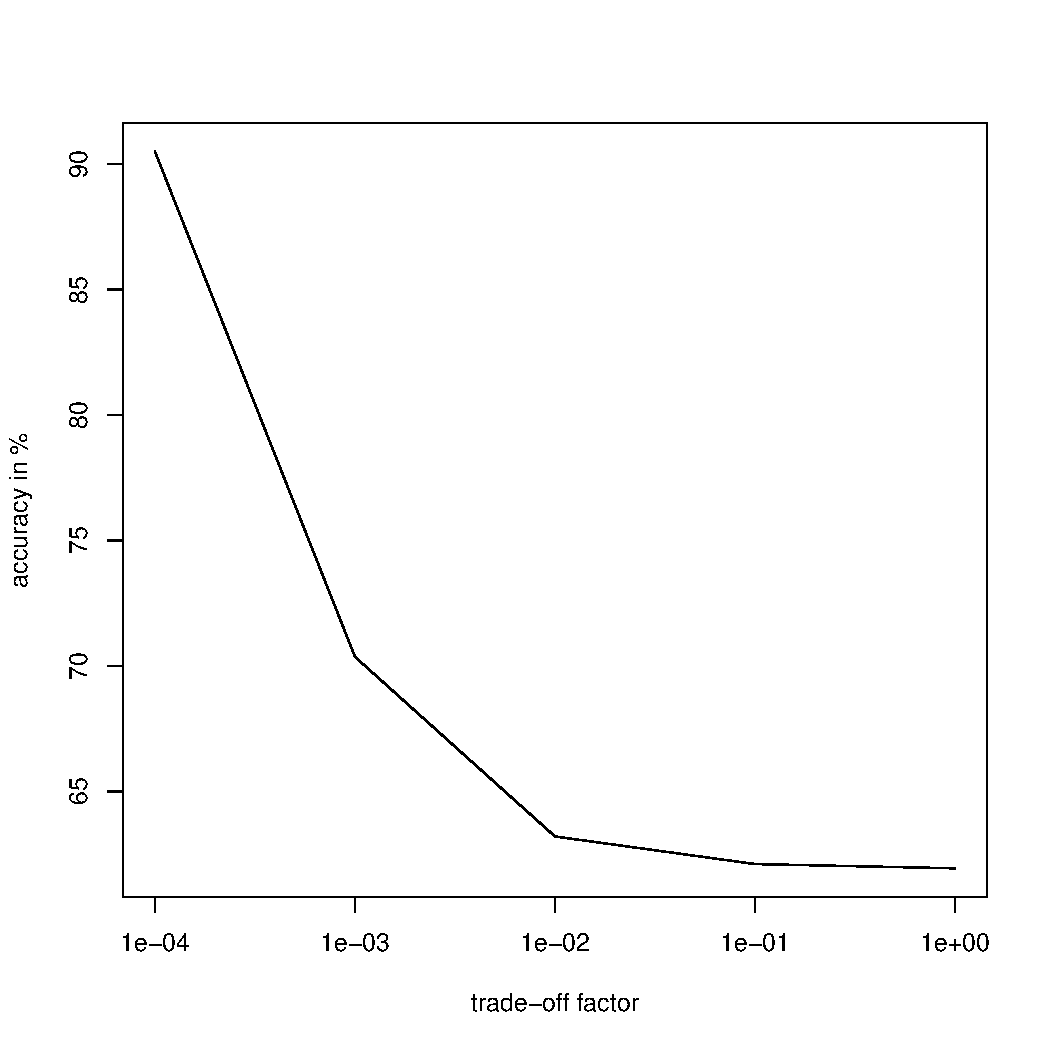
\includegraphics[width=0.6\textwidth]{../dia/accuracy.pdf} }}
    \qquad
    \subfloat[runtime for $\lambda$]{{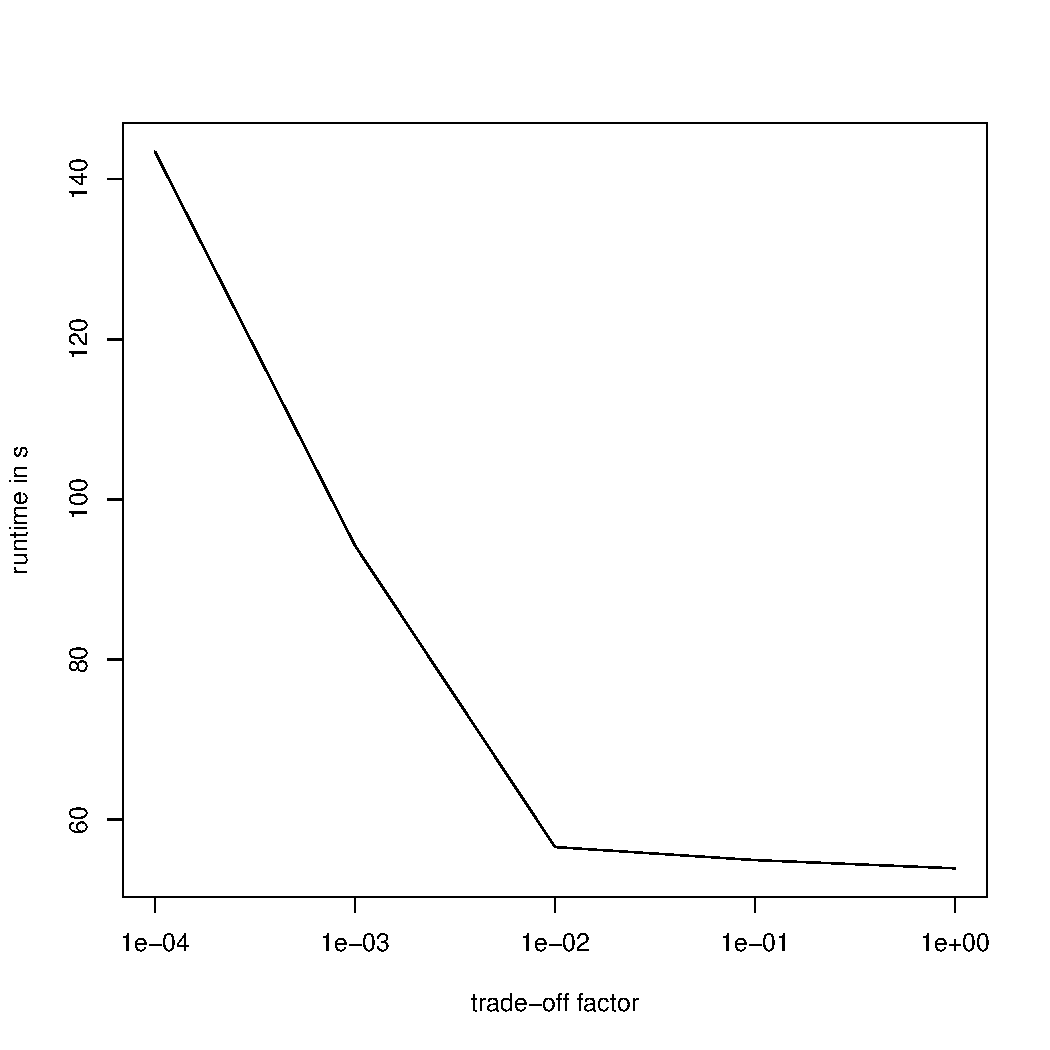
\includegraphics[width=0.6\textwidth]{../dia/runtime.pdf} }}
    \caption{runtime and accuracy for given $lambda$}
    \label{fig:ar}
\end{figure}
Figure \ref{fig:ar} shows the impact of $\lambda$ for the average accuracy and the average runtime. While the values for high $\lambda$ varies slightly, an enormous difference can be observed for small $\lambda$ ($0.0001$ and $0.001$). Considering the smallest and the largest $\lambda$ in this experimental design ($0.0001$ and $1$), a reduction of the runtime by almost $30$ seconds can be achieved if we use large $\lambda$ for pruning. However, we will lose almost $30\%$ accuracy as well.


\section{Conclusion and Outlook}

In this work, we presented a parse chart-like construct for PLCFRS in form of (pruned) derivation graphs and an approach to train pruning policies for PLCFRS by using an user-defined trade-off factor. We investigated the impact of the trade-off factor in case of the accuracy and in case of the runtime for weighted deductive parsing for PLCFRS. The parser works with PLCFRS with any fanout size and the training allows to use redefined features or self defined features.

For the calculation of the reward, we used one fixed computation method, schematically $reward = accuracy - \lambda * runtime$, as proposed in \cite{vieira17}.
However, it could be interesting to see in future work, how the resulting pruning policies will change if not only the trade-off factor $\lambda$ would be a variable but the computing method for the reward as well.
In the described setup, we used the fixed features as defined in chapter 6. New features could be added easily for investigating its impact on the pruning policies.
Furthermore, the used parser works in an exhausting manner, speed ups in the parsing process can be reached by implementing an non-exhaustive parser or even one with taking normalized PLCFRS into account.


\section{References}
\nocite{*}
\printbibliography[heading=none]

\end{document}